\documentclass[12pt, twoside]{article}
\documentclass[12pt, twoside]{article}
\usepackage[letterpaper, margin=1in, headsep=0.2in]{geometry}
\setlength{\headheight}{0.6in}
%\usepackage[english]{babel}
\usepackage[utf8]{inputenc}
\usepackage{microtype}
\usepackage{amsmath}
\usepackage{amssymb}
%\usepackage{amsfonts}
\usepackage{siunitx} %units in math. eg 20\milli\meter
\usepackage{yhmath} % for arcs, overparenth command
\usepackage{tikz} %graphics
\usetikzlibrary{quotes, angles}
\usepackage{graphicx} %consider setting \graphicspath{{images/}}
\usepackage{parskip} %no paragraph indent
\usepackage{enumitem}
\usepackage{multicol}
\usepackage{venndiagram}

\usepackage{fancyhdr}
\pagestyle{fancy}
\fancyhf{}
\renewcommand{\headrulewidth}{0pt} % disable the underline of the header
\raggedbottom
\hfuzz=2mm %suppresses overfull box warnings

\usepackage{hyperref}
\usepackage{float}

\fancyhead[LE]{\thepage}
\fancyhead[RO]{\thepage \\ First and last name: \hspace{2.5cm} \,\\ Section: \hspace{2.5cm} \,}
\fancyhead[LO]{BECA / Dr. Huson / Regents Prep: Graphs\\* 27 November 2024}

\begin{document}

\subsubsection*{3.10 Do Now: Graphing 4th degree polynomials}
\begin{enumerate}
\item On the grid below, graph the function $f(x) = x^{3} - 6x^{2} + 9x + 6$ on the domain $-1\leq x \leq 4$. 
  \begin{enumerate}
      \item Mark and label the $x$-intercepts. 
      \item Write the function in factored form. \vspace{1.5cm}
      \item Characterize the end behavior of the function. Use the notation \\
      ``as $x \rightarrow \pm \infty$ $y \rightarrow\pm \infty$"    
      \item Mark and label the relative minimum point as an ordered pair.
  \end{enumerate} \hspace{2cm}
  
    \begin{center}
    \begin{tikzpicture}[scale=.635]
      \draw [help lines] (-10,-10) grid (10,10);
      \draw [thick, ->] (-10.2,0) -- (10.4,0) node [below right] {$x$};
      \draw [thick, ->] (0,-10.2)--(0,10.4) node [left] {$y$};
      %\draw[thick, <->,smooth, domain=-3.3:2.1] plot (\x, {2.5*(\x)^2 + 3*\x - 7});
    \end{tikzpicture}
    \end{center}

\newpage
\item Circle the equations that are an identities.
    \begin{multicols}{2}
      \begin{enumerate}
        \item \(x^2 - y^2 = (x - y)(x+y)\)
        \item \((x + y)^2 = x^2 + 2xy + y^2\)
        \item \(x^3 - y^3 = (x - y)(x^2 - xy + y^2)\)
        \item \(x^3 + y^3 = (x + y)(x^2 - xy + y^2)\)
      \end{enumerate}
    \end{multicols}

\item Write a recursive definition of the sequence $a_1 = 10$, $a_2 = 1$, $a_3 = 0.1$, $a_4 = 0.01, \ldots$ \vspace{2cm}
    
\item Write down the solutions to the equation $x(3x+4)(x +1)(x - 5) = 0$ \vspace{1.5cm} 

\item Graphed is $y = f(x)$. Write the function in factored form. 
    \begin{multicols}{2}
    \begin{enumerate}
      \item Is the leading coefficient positive or negative?
      \item What is its end behavior?
      \item What is the degree of the polynomial?
    \end{enumerate}
    \begin{flushright}
    \begin{tikzpicture}[xscale=1, yscale=0.25]
      \draw [thick, ->] (-3.2,0) -- (3,0) node [above] {$x$};
      \draw [thick, ->] (0,-9.2)--(0,10) node [right] {$y$};
      %\foreach \x in {-3,...,3} \draw (\x cm,12pt) -- (\x cm,-12pt) node[below] {$\x$};
      %\foreach \y in {-8,-6,4,8} \draw (3pt,\y cm) -- (-3pt,\y cm) node[left] {$\y$};
      \draw [thick, <->,smooth,samples=20,domain=-3.3:2.4] plot(\x,{-(\x-2)*(\x+1)*(\x+3)});
    \end{tikzpicture}
    \end{flushright}
    \end{multicols} \vspace{1cm}

\item If the diameter of a storm is 30 miles, how long might it last in hours? Use the formula
$D^3 = 216 T^2$ where $D$ is the diameter in miles and $T$ is the duration in hours.

\end{enumerate}
\end{document}